\section{The Time-Independent Schr\"odinger Equation (TISE)}


\begin{itemize}
    \item Let's recall the ordinary SE, where we will write the wavefunction now as capital $\Psi$.
        \begin{equation}
            i\hbar\diffp{\Psi}{t} = -\frac{\hbar^2}{2m} \diffp[2]{\Psi}{x} + V\Psi.
        \end{equation}
    \item Now that we have explored the properties of this equation, we are now interested in what solutions to it might look like. As a PDE, our first move as physicists should be \textit{separation of variables}. Let's assume a solution like $\Psi(x,t) = \phi(t)\psi(x)$, and plug it in:
        \begin{equation}
            i\hbar \psi \diff{\phi}{t} = -\frac{\hbar^2}{2m} \phi \diff[2]{\psi}{x} + V\phi\psi.
        \end{equation}
    \item Dividing both sides by $\phi\psi$, we get
        \begin{equation}
            i\hbar \frac{1}{\phi} \diff{\phi}{t} = -\frac{\hbar^2}{2m} \frac{1}{\psi} \diff[2]{\psi}{x} + V.
        \end{equation}
    \item Now, since we have two completely independent quantities on either side, they must be equal to a constant, which we will call $E$ (this will be identified as the energy):
    \renewcommand{\arraystretch}{1.2}
        \begin{equation}
        \begin{cases}
            \diff{\phi}{t} = -\frac{iE}{\hbar} \phi, \\
            -\dfrac{\hbar^2}{2m}\diff[2]{\psi}{x} + V\psi = E\psi.\label{TISE}
        \end{cases}
        \end{equation}
    \renewcommand{\arraystretch}{1}
    \item The $t$ equation is super simple:
        \begin{equation}
            \phi(t) = e^{-iEt/\hbar},
        \end{equation}
        where we have just chosen to absorb the constant into $\psi$.
    \item The $x$ equation is unsolvable until we know what our potential $V$ is; Eq.~\eqref{TISE} is the \textbf{time-independent Schr\"odinger Equation (TISE)}.
    \item Upon further examination, we can identify it with the Hamiltonian operator we found earlier:
        \begin{equation}
            \hat{H} = -\frac{\hbar^2}{2m} \diff[2]{}{x} + V,
        \end{equation}
        so the TISE becomes
        \begin{equation}
            \hat{H}\psi = E\psi,
        \end{equation}
        or an eigenvalue equation.
\end{itemize}

\sep

\begin{itemize}
    \item To motivate why we'd be interested in such solutions, since it seems unlikely that such a wild assumption from the beginning can provide any sort of meaninful results, we can make the following observations: first, these are \textit{stationary} states. Now, the probability density is time-independent, as we saw before, and so are our expectation values. Let's show the latter:
        \begin{equation}
            \braket{x} = \bra{\Psi}x\ket{\Psi} = \int\Psi^* x \Psi \;\dd x = \int e^{iEt/\hbar}\psi x e^{-iEt/\hbar}\psi \;\dd x = \int \psi^* x \psi \;\dd x.
        \end{equation}
    \item The same will be true for the other expectation values that we have looked at thus far. So, when looking at these values, we might as well just drop the time-dependent factor and only focus on the time-independent solutions to determine these values. Hence, these TISE solutions, since they are easier to solve for, are useful in that regard.
    \item Additionally, we have that such solutions, upon measurement, give a definite value for the energy, i.e. $\sigma_H = 0$. To show this, let's calculate $\braket{\hat{H}}$ and $\braket{\hat{H}}$:
        \begin{equation}
            \braket{\hat{H}} = \int \psi^* \hat{H} \psi \;\dd x,
        \end{equation}
        but from the TISE, we know that $\hat{H}\psi = E\psi$, so
        \begin{equation}
            \braket{\hat{H}} = E\int \psi^*\psi \;\dd x = E\int \abs{\psi}^2 \;\dd x = E.
        \end{equation}
    \item Next, we have that
        \begin{equation}
            \hat{H}^2\psi = \hat{H} \left(\hat{H}\psi\right) = E \left(\hat{H} \psi\right) = E^2\psi,
        \end{equation}
    \item So,
        \begin{equation}
            \braket{\hat{H}^2} = \int \psi^* \hat{H}^2 \psi \;\dd x = E^2 \int \psi^* \psi \;\dd x = E^2.
        \end{equation}
    \item Therefore,
        \begin{equation}
            \sigma_H = \sqrt{\braket{\hat{H}^2} - \braket{\hat{H}}^2} = \sqrt{E^2 - E^2} = 0.
        \end{equation}
    \item Hence, we have shown that there is zero variance in the value of $E$ resulting from the Hamiltonian operator, meaning that the energy is the same for every measurement.
    \item Additionally, it can be shown that when solving for the TISE, we actually get an infinite number of solutions corresponding to the infinite number of possible definite energy states. Further, since the SE is linear, the sum of all of these solutions is equal to the full, general solution. More formally, the $n$th solution is given by
        \begin{equation}
            \Psi_n(x,t) = \psi_n(x) e^{-iE_n t/\hbar},
        \end{equation}
        so the full solution would be:
        \begin{equation}
            \Psi(x,t) = \sum_n c_n \psi_n(x) e^{-iE_nt/\hbar} = \sum_n c_n \Psi_n(x,t),
        \end{equation}
        where the $c_n$'s are constants. For $t=0$, when one is looking to normalize the wavefunction, this reduces to
        \begin{equation}
            \Psi(x,0) = \sum_n c_n \psi_n(x).
        \end{equation}
\end{itemize}


\begin{example}
    Prove the following statement: For normalizable solutions, $E$ must be real.

    \begin{itemize}
        \item First, let's start by assuming $E = E_0 + iE_1$. Then, our general solution becomes:
            \begin{equation}
                \Psi = A\psi e^{-i(E_0 + iE_1)t/\hbar} = A\psi e^{-iE_0t/\hbar} \cdot e^{E_1t/\hbar}.
            \end{equation}
            Let's normalize this:
            \begin{align}
                \int \abs{\Psi}^2 \;\dd x &= A^2 \int \psi^*\psi e^{-iE_0t/\hbar}e^{iE_0t/\hbar} \cdot e^{E_1t/\hbar} \cdot e^{E_1t/\hbar} \;\dd x \\ 
                &= A^2 e^{2E_1t/\hbar} \int \abs{\psi}^2 \;\dd x \\
                &= A^2 e^{2E_1t/\hbar} = 1.
            \end{align}
            Now, we have already proved that a function normalized at one particular time stays normalized for all other times. However, here we have a time-dependent term equalling a constant. Therefore, for our function to be able to be normalized, we must have $E_1 = 0$ to remove the time-dependent term. $E_1$ was the imaginary term, hence, the separation constant cannot be imaginary.
    \end{itemize}
\end{example}


\sep


\subsection*{The Infinite Square Well}

\begin{itemize}
    \item With some of the formalism out of the way we can start looking at solving some specific examples using the TISE. The first of these is the infinite square well, in which a particle is confined to some region (a ``well'') by an infinite potential on either side. In this particular example, we imagine a potential
        \begin{equation*}
            V = 
                \begin{alignedat}{1}
                \begin{cases}
                    0,\qquad\quad &0 \leq x \leq a, \\
                    \infty & \text{elsewhere}.
                \end{cases}
            \end{alignedat}
        \end{equation*}
    \item Notably, this is not time-dependent, meaning we can use the TISE. Now, since the potential is infinite outside the well, there is zero chance the particle could end up there, so $\psi=0$ outside. Inside, we have a zero potential, so the TISE reduces to:
        \begin{equation*}
            -\frac{\hbar^2}{2m}\diff[2]{\psi}{x} = E\psi.
        \end{equation*}
        Rewriting:
        \begin{equation*}
            \diff[2]{\psi}{x} + \frac{2mE}{\hbar^2}\psi = 0,
        \end{equation*}
        or, defining
        \begin{equation*}
            k \equiv \frac{\sqrt{2mE}}{\hbar},
        \end{equation*}
        we can write this as
        \begin{equation*}
            \diff[2]{\psi}{x} + k^2\psi = 0.
        \end{equation*}
    \item However, negative energy states are possible, right? In this case, actually, this is not the case, and it is a small exercise to show that for a normalizable stationary state, the minimum allowed energy must exceed the potential. Let's show this, since its easy.
    \item We first rewrite the TISE like so:
        \begin{equation*}
            \diff[2]{\psi}{x} = \frac{2m}{\hbar^2} \left[V(x) - E\right]\psi.
        \end{equation*}
        Let's consider when $E<V$. In this case, we have that both the wavefunction and its second derivative are of the same sign. So, if our wavefunction itself is positive, then the second derivative must be positive. A positive function with a positive second derivative means that it will be curving up away from the $x$-axis, getting larger and larger, and vice versa for a negative wavefunction. So, in either case, the wavefunction either increases to infinity or decreases to infinity. The only other way for this not to be the case is if the wavefunction is zero, but that also is not normalizable.
    \item Now that we have shown that, we can more safely place the energy within the square root as shown above.
    \item The solutions to our TISE for the infinite square well are just sines and cosines:
        \begin{equation*}
            \psi(x) = A\cos(kx) + B\sin(kx).
        \end{equation*}
        We now just quote results from future chapters, the main one being that the wavefunction must be continuous. This seems intuitive, but it'll be proved later supposedly. Due to this, the wavefunction at the end points of the well must be zero:
        \begin{equation*}
            \psi(0) = A\cos0 + B\sin0 = A = 0,
        \end{equation*}
        so we have eliminated the $\cos$ part and just have
        \begin{equation*}
            \psi(x) = A\sin(kx),
        \end{equation*}
        where I have just relabeled the constant to be $A$.
    \item Next, we apply the other boundary condition:
        \begin{equation*}
            \psi(a) = A\sin(ka) = 0.
        \end{equation*}
        Here, though, we can either set $A=0$ or $\sin(ka)=0$. We don't want to do $A=0$, the trivial solution, because such a wavefunction, as just mentioned, is not normalizable. So, we must set $\sin(ka)=0$. This means that the quantity $ka$ must be an integer multiple of $\pi$ (and cannot be zero!):
        \begin{equation*}
            ka = n\pi \ \rightarrow\ k = \frac{n\pi}{a}.
        \end{equation*}
    \item But wait... Recalling how we defined $k$ in the first place:
        \begin{gather*}
            \frac{n\pi}{a} = \frac{\sqrt{2mE}}{\hbar}, \\
            \frac{n^2\pi^2}{a^2} = \frac{2mE}{\hbar^2}, \\
            \rightarrow \boxed{E = \frac{n^2\pi^2\hbar^2}{2ma}.}
        \end{gather*}
    \item What we have just shown is that the energy values for this system can only take on discrete values, as dictated by the $n^2$! This is extremely unexpected from a classical standpoint.
    \item Now back to our wavefunction, we can now normalize to determine $A$:
        \begin{align*}
            A^2 \int_0^a \sin^2(kx) \;\ddx &= \frac{A^2}{2} \int_0^a \left(1 - \cos(2kx)\right) \;\ddx, \\
            &= \frac{A^2}{2} \left[x - \frac{1}{2k}\sin(kx)\right]_0^a, \\
            &= \frac{A^2}{2} \left[a - \frac{2a}{n\pi}\sin(2n\pi)\right], \\
            &= \frac{A^2 a}{2} = 1, \\
            \rightarrow\ \Aboxed{A = \sqrt{\frac{2}{a}}.}
        \end{align*}
        Our wavefunction is, therefore:
        \begin{equation}
            \psi_n(x) = \sqrt{\frac{2}{a}} \sin\left(\frac{n\pi x}{a}\right),\label{InfSquareWellTISol}
        \end{equation}
        where I have added the subscript $n$ to signify that we now have an infinite set of discretized solutions.
\end{itemize}

\sep

\begin{itemize}
    \item We can now quote a couple of properties about our infinite set of solutions and the TISE in general:
    \begin{enumerate}
        \item Our set of solutions alternate between even and odd. For instance, $\psi_1$ is even, $\psi_2$ is odd, $\psi_3$ is even again, and so on.
        \item Each successive increase in energy adds one node to the resulting plots of the energy. A node is basically a crossing of the $x$-axis by the wave.
        \item They are mutually orthogonal to each other, meaning that
            \begin{equation}
                \int \psi_i(x)^* \psi_j(x) \;\ddx = \delta_{ij}.\label{WavefunctionOrthogonality}
            \end{equation}
            This captures that when $i=j$, the wavefunctions are the same and it is just the normalization condition, but if $i\neq j$, then the result is zero. This is the definition of orthogonality, and it means that the set itself is \textbf{orthonormal}.
        \item The set is \textbf{complete}, meaning that we can express any function $f(x)$ by using our solutions in a linear combination:
            \begin{equation*}
                f(x) = \sum_n c_n \sqrt{\frac{2}{a}}\sin\left(\frac{n\pi x}{a}\right).
            \end{equation*}
            This shouldn't be shocking, since we have basically just constructed a Fourier series, and we know from \textbf{Dirichlet's Theorem} that we can represent any function as a Fourier series.
    \end{enumerate}
\end{itemize}

\sep

\begin{itemize}
    \item Lastly, we can assemble the full time-dependent solutions by tacking on the exponential time factor:
        \begin{equation*}
            \Psi_n(x,t) = \sqrt{\frac{2}{a}} \sin\left(\frac{n\pi x}{a}\right) e^{-i(n^2\pi^2\hbar/2ma^2)t}.
        \end{equation*}
        And, again, the most general solution is a linear combination, so:
        \begin{equation}
            \boxed{\Psi(x,t) = \sqrt{\frac{2}{a}} \sum_n c_n \sin\left(\frac{n\pi x}{a}\right)e^{-i(n^2\pi^2\hbar/2ma^2)t}.}\label{InfSquareWellFullSolution}
        \end{equation}
\end{itemize}

\sep

\begin{itemize}
    \item The general way to solve a problem using this, is to take the given initial wavefunction $\Psi(x,0)$, then from the completeness of the $\psi_n$'s, we can use our initial wavefunction to find the $c_n$'s using Fourier's trick:
        \begin{equation}
            c_n = \int \psi_n^{\dagger}(x) \Psi(x,0) \;\ddx,\label{InfSquareWellStartingPoint}
        \end{equation}
        and from there, we can assemble the full solution using Eq.~\eqref{InfSquareWellFullSolution}.
\end{itemize}

\begin{example}
    Before moving on to more series examples, let's first explore further our solutions to this infinte square well. Let's calculate the expectation values of $x$, $x^2$, $p$, and $p^2$ along with their uncertainties for the $n$th state.

    \begin{itemize}
        \item Since the expectation values are time-independent (either way, the time-dependent exponential cancels), we can just do:
            \begin{align*}
                \braket{x} &= \int \psi_n^* x \psi \;\ddx = \frac{2}{a}\int_0^a x \sin^2\left(\frac{n\pi x}{a}\right) \;\ddx, \\
                &= \frac{1}{a} \int_0^a x \left[1 - \cos\left(\frac{2n\pi x}{a}\right)\right]\;\ddx, \\
                &= \frac{1}{a}\int_0^a x\;\ddx - \frac{1}{a}\int_0^a x\cos\left(\frac{2n\pi x}{a}\right)\;\ddx, \\
                &= \frac{a}{2} - \frac{1}{a}\left\{\frac{xa}{2n\pi}\sin\left(\frac{2n\pi x}{a}\right)\Big|_0^a - \frac{a}{2n\pi} \int_0^a \sin\left(\frac{2n\pi x}{a}\right)\;\ddx\right\}.
            \end{align*}
            The first term in the braces vanishes, so we have
            \begin{align*}
                \braket{x^2} &= \frac{a}{2} - \frac{1}{a} \left[\frac{a^2}{4n^2\pi^2} \cos\left(\frac{2n\pi x}{a}\right)\right]_0^a, \\
                &= \frac{a}{2} - \frac{a}{4n^2\pi^2}\left[\cos(2n\pi)-1\right].
            \end{align*}
            Cosine of an integer multiple of $2\pi$ is always 1, so the entire term with brackets vanishes, leaving:
            \begin{equation*}
                \braket{x} = \frac{a}{2}.
            \end{equation*}
        \item Since we got this from the full time-dependent equation we can say
            \begin{equation*}
                \braket{p} = \diff[]{\braket{x}}{t} = 0.
            \end{equation*}
        \item Now,
            \begin{align*}
                \braket{x^2} &= \frac{1}{a}\int_0^a x^2\;\ddx - \frac{1}{a} \int_0^a x^2\cos\left(\frac{2\pi x}{a}\right)\;\ddx, \\
                &= \frac{a^2}{3} + \frac{1}{a} \left\{\frac{ax^2}{2n\pi}\sin\left(\frac{2n\pi x}{a}\right)\Big|_0^a - \frac{a}{n\pi}\int_0^a x\sin\left(\frac{2n\pi x}{a}\right) \;\ddx\right\}.
            \end{align*}
            Again, the first term in braces vanishes;
            \begin{align*}
                \braket{x^2} &= \frac{a^2}{3} + \frac{1}{n\pi}\int_0^a x\sin\left(\frac{2n\pi x}{a}\right)_0^a \;\ddx, \\
                &= \frac{a^2}{3} + \frac{1}{n\pi}\left\{-\frac{xa}{2n\pi}\cos\left(\frac{2n\pi x}{a}\right)\Big|_0^a - \frac{a}{2n\pi}\int_0^a \cos\left(\frac{2n\pi x}{a}\right)\;\ddx\right\}.
            \end{align*}
            The integral will give a sine, evaluated over the same limits as before, and will vanish. So
            \begin{align*}
                \braket{x^2} &= \frac{a^2}{3} + \frac{1}{n\pi} \left(\frac{-a^2}{2n\pi}\right), \\
                &= \frac{a^2}{3} - \frac{a^2}{2n^2\pi^2}, \\
                \braket{x^2} &= a^2 \left(\frac{1}{3} - \frac{1}{2n^2\pi^2}\right).
            \end{align*}
        \item Next,
            \begin{align*}
                \braket{p^2} &= \int \psi_n^*(x) \left(-i\hbar \diff[2]{}{x}\right)^2 \psi_n(x) \;\ddx, \\
                &= -\hbar^2 \int \psi_n^*(x) \diff[2]{\psi}{x} \;\ddx.
            \end{align*}
            From our TISE, we know that
            \begin{equation*}
                \diff[2]{\psi}{x} = -k^2\psi = -\frac{2mE}{\hbar^2}\psi = -\frac{2m}{\hbar^2} \left(\frac{n^2\pi^2\hbar^2}{2ma^2}\right)\psi = -\frac{n^2\pi^2}{a},
            \end{equation*}
            so
            \begin{equation*}
                \braket{p^2} = \frac{n^2\pi^2\hbar^2}{a^2}\int \abs{\psi_n}^2 \;\ddx = \frac{n^2\pi^2\hbar^2}{a^2}.
            \end{equation*}
        \item Next,
            \begin{align*}
                \sigma_x &= \sqrt{a^2\left(\frac{1}{3} - \frac{1}{2n^2\pi^2}\right) - \left(\frac{a}{2}\right)^2}, \\
                \sigma_p &= \sqrt{\frac{n^2\pi^2\hbar^2}{a^2}} = \frac{n\pi\hbar}{a}.
            \end{align*}
            Putting them into the uncertainty relation:
            \begin{align*}
                \sigma_x \sigma_p &= \hbar \sqrt{\frac{\pi^2n^2}{3} - \frac{1}{2} - \frac{n^2\pi^2}{4}}, \\
                &= \frac{\hbar}{2} \sqrt{\frac{4\pi^2n^2}{3} - 2 - n^2\pi^2}, \\
                &= \frac{\hbar}{2} \sqrt{\frac{n^2\pi^2}{3} - 2} \geq \frac{\hbar}{2}.
            \end{align*}
            This is satisfied since $\pi^2/3 > 3$, and $n^2 > 1$, so $n^2\pi^2/3 > 2$ always.
        \item The value of $n$ that brings this closest to the limit is actually the smallest and most likely value, $n=1$. Larger values make the value in the square root larger, so the smallest possible value is the right one.
    \end{itemize}
\end{example}




\begin{example}
    A particle in an infinite square well has the initial wave function 

    \begin{equation}
        \Psi(x,0) =
            \begin{alignedat}{1}
            \begin{cases}
                Ax \qquad & 0 \leq x \leq a/2, \\
                A(a-x) & a/2 \leq x \leq a.
            \end{cases}
            \end{alignedat}
    \end{equation}

    Find $A$, then find $\Psi(x,t)$.

    \sep

    \begin{itemize}
        \item First, we just normalize the wave function to find $A$:
            \begin{align*}
                \braket{\psi | \psi} &= A^2 \int_0^{a/2} x^2 \;\ddx + A^2 \int_{a/2}^a (a-x)^2 \;\ddx, \\
                &= A^2 \left[ \frac{1}{2}\left(\frac{a}{2}\right)^3 + \int_{a/2}^a x^2\;\ddx - 2a\int_{a/2}^a x\;\ddx + a^2 \int_{a/2}^a \;\ddx \right], \\
                &= A^2 \left\{ \frac{a^3}{24} + \frac{1}{3}\left[a^3 - \left(\frac{a}{2}\right)^3\right] - a\left[a^2 - \left(\frac{a}{2}\right)^2\right] + a^2 \left(a - \frac{a}{2}\right) \right\}, \\
                &= A^2 \left[\frac{a^3}{24} + \frac{a^3}{3}\left(\frac{7}{8}\right) - a^3 \left(\frac{3}{4}\right) + a^3 \left(\frac{1}{2}\right)\right], \\
                &= A^2a^3 \left(\frac{1}{3} - \frac{3}{4} + \frac{1}{2}\right) = A^2a^3 \left(\frac{4}{12} - \frac{9}{12} + \frac{6}{12}\right) = \frac{A^2a^3}{12} = 1,
            \end{align*}
            so
            \begin{equation*}
                \boxed{A = \sqrt{\frac{12}{a^3}}.}
            \end{equation*}
        \item To find the general solution, we can use Eq.~\eqref{InfSquareWellStartingPoint} and substitute $\psi_n$ with Eq.~\eqref{InfSquareWellTISol} and $\Psi(x,0)$ with our given wavefunction:
            \begin{equation*}
                c_n = \sqrt{\frac{2}{a}}\sqrt{\frac{12}{a^3}} \left[\int_0^{a/2} x\sin\left(\frac{n\pi x}{a}\right)\;\ddx + \int_{a/2}^a (a-x)\sin\left(\frac{n\pi x}{a}\right) \;\ddx\right].
            \end{equation*}
            Looking at the first integral first:
            \begin{align*}
                \int_0^{a/2} x\sin\left(\frac{n\pi x}{a}\right)\;\ddx &= \left[-\frac{xa}{n\pi}\cos\left(\frac{n\pi x}{a}\right)\right]_0^{a/2} + \frac{a}{n\pi}\int_0^{a/2} \cos\left(\frac{n\pi x}{a}\right) \;\ddx, \\
                &= -\frac{a^2}{2n\pi}\cos\left(\frac{n\pi}{2}\right) + \frac{a^2}{n^2\pi^2}\sin\left(\frac{n\pi}{2}\right).
            \end{align*}
            Now for the second integal:
            \begin{equation*}
                \int_{a/2}^a (a-x)\sin\left(\frac{n\pi x}{a}\right) \;\ddx = a\int_{a/2}^a \sin\left(\frac{n\pi x}{a}\right) \;\ddx - \int_{a/2}^a x\sin\left(\frac{n\pi x}{a}\right)\;\ddx,
            \end{equation*}
            \begin{align*}
                &= \left[-\frac{a^2}{n\pi} \cos\left(\frac{n\pi x}{a}\right)\right]_{a/2}^a - \left[-\frac{xa}{n\pi} \cos\left(\frac{n\pi x}{a}\right)\right]_{a/2}^a + \left[\frac{a^2}{n^2\pi^2} \sin\left(\frac{n\pi x}{a}\right)\right]_{a/2}^a, \\
                &= -\frac{a^2}{n\pi} \left[\cos(n\pi) - \cos\left(\frac{n\pi}{2}\right)\right] + \frac{a}{n\pi} \left[a\cos(n\pi) - \frac{a}{2}\cos(\frac{n\pi}{2})\right] - \frac{a^2}{n^2\pi^2}\left[\sin(n\pi) - \sin\left(\frac{n\pi}{2}\right)\right], \\
                &= \frac{a^2}{2n\pi}\cos\left(\frac{n\pi}{2}\right) + \frac{a^2}{n^2\pi^2}\sin\left(\frac{n\pi}{2}\right).
            \end{align*}
            Adding the two together,
            \begin{align*}
                c_n &= \sqrt{\frac{24}{a^4}} \left[-\frac{a^2}{2n\pi}\cos\left(\frac{n\pi}{2}\right) + \frac{a^2}{n^2\pi^2}\sin\left(\frac{n\pi}{2}\right) + \frac{a^2}{2n\pi}\cos\left(\frac{n\pi}{2}\right) + \frac{a^2}{n^2\pi^2}\sin\left(\frac{n\pi}{2}\right)\right], \\
                &= \frac{4\sqrt{6}}{n^2\pi^2}\sin\left(\frac{n\pi}{2}\right), \\
                &=
                    \begin{alignedat}{2}
                    \begin{cases}
                        \frac{(-1)^{(n-1)/2}4\sqrt{6}}{n^2\pi^2} \quad &\text{odd}\ n, \\
                        0 & \text{even}\ n.
                    \end{cases}
                \end{alignedat}
            \end{align*}
            At last, then, our general solution is
            \begin{equation*}
                \boxed{\Psi(x,t) = \frac{4\sqrt{6}}{\pi^2} \sum^{\infty}_{n=1,3,5,\ldots} \frac{(-1)^{(n-1)/2}}{n^2} \sin\left(\frac{n\pi x}{a}\right)e^{-i(n^2\pi^2\hbar)t/(2ma^2)}.}
            \end{equation*}
    \end{itemize}

    \sep 

    Now, what is the probability that a measurement of the energy will yield $E_1$?

    \begin{itemize}
        \item We know that the probability of measuring state $n$ is $\abs{c_n}^2$:
            \begin{equation*}
                P(E = E_1) = \left( \frac{(-1)^{(1-1)/2} 4\sqrt{6}}{1^2\pi^2} \right)^2 = \frac{96}{\pi^4} \approx 0.9855.
            \end{equation*}
    \end{itemize}

    \sep 

    Lastly, find $\braket{H}$, using the formula

    \begin{equation}
        \braket{H} = \sum_{n=1}^{\infty} \abs{c_n}^2 E_n.
    \end{equation}

    \begin{itemize}
        \item Let's just plug in:
            \begin{equation*}
                \braket{H} = \sum_{n=1,3,5,\ldots}^{\infty} \left(\frac{(-1)^{(n-1)/2} 4\sqrt{6}}{n^2\pi^2}\right)^2 \left(\frac{n^2\pi^2\hbar^2}{2ma^2}\right) = \frac{48\hbar}{ma^2\pi^2} \sum_{n=1,3,5,\ldots}^{\infty} \frac{1}{n^2}.
            \end{equation*}
            The infinite series turns out to be $\pi^2/8$, so the expectation value for the energy is:
            \begin{equation*}
                \boxed{\braket{H} = \frac{6\hbar^2}{ma^2}.}
            \end{equation*}
    \end{itemize}
\end{example}



\subsection*{The Simple Harmonic Oscillator}



\begin{itemize}
    \item The \textbf{simple harmonic oscillator} (SHO) involves a force acting on a particle that is directly and oppositely proportional to its distance from some equilibrium position:
        \begin{equation*}
            F \propto -x.
        \end{equation*}
        If we call the proportionality constant $k$, we have \textit{Hooke's Law}:
        \begin{align*}
            F &= -kx, \\
            m\diff[2]{x}{t} &= -kx, \\
            \diffp[2]{x}{t} + \frac{k}{m}x &= 0, \\
            \diffp[2]{x}{t} + \omega^2x &= 0,
        \end{align*}
        where $\omega = \sqrt{k/m}$.
    \item Solutions to this equation are waves.
    \item Now we know that for conservative forces, $F_x = -\grad_x V$, or $V = -\int F\;\ddx$. Thus,
        \begin{equation*}
            V = \int kx\;\ddx = \frac{1}{2}m\omega^2x^2.
        \end{equation*}
    \item Bringing this to a quantum system, we note that this potential is time-independent, meaning we can apply the TISE:
        \begin{equation*}
            -\frac{\hbar^2}{2m}\diff[2]{\psi}{x} + \frac{1}{2}m\omega^2x^2 \psi = E\psi.
        \end{equation*}
    \item This is super tricky to solve, so we will use an ad hoc solution that people a long time ago found the hard way. The first step in this clever method is to write our TISE like so:
        \begin{align*}
            &\frac{1}{2m} \left[ -\hbar^2 \diff[2]{\psi}{x} + m^2\omega^2x^2 \psi \right] = E\psi, \\
            &\frac{1}{2m} \left[ \left( \frac{\hbar}{i}\diff{}{x} \right)^2 + (m\omega x)^2 \right] \psi = E\psi.
        \end{align*}
        Now let's define 
        \begin{equation}
            \hat{a}_{\pm} = \frac{1}{\sqrt{2m}} \left( \frac{\hbar}{i} \diff{}{x} \pm im\omega x \right),
        \end{equation}
    \item Ordinarily we could factor our TISE simply into $\hat{a}_{\pm}$, but since $\hat{a}$ is an operator, it is not so simple. Let's examine these operators using a test function $f(x)$. First,
        \begin{align*}
            \hat{a}_-\hat{a}_+ f(x) &= \frac{1}{2m}\left[ \left( \frac{\hbar}{i}\diff{}{x} \right) - im\omega x \right]\left[ \left( \frac{\hbar}{i}\diff{}{x} \right) + im\omega x \right]f(x), \\
            &= \frac{1}{2m} \left[ \left( \frac{\hbar}{i}\diff{}{x} \right)^2f(x) + \hbar m \omega \diff{}{x}[xf(x)] -\hbar m\omega x\diff{}{x}[f(x)] + (m\omega x)^2 f(x) \right].
        \end{align*}
        We need the product rule for the second term. We can see that we will end up with a term identical to the third term but positive, so those cancel, meaning all we are left with is a term that has $\dd x/\dd x$, which is 1:
        \begin{align*}
            \hat{a}_-\hat{a}_+ f(x) &= \frac{1}{2m} \left[ \left( \frac{\hbar}{i}\diff[]{}{x} \right)^2f(x) + (m\omega x)^2f(x) + \hbar m\omega f(x) \right], \\
            &= \frac{1}{2m} \left[ \left( \frac{\hbar}{i}\diff[]{}{x} \right)^2 + (m\omega x)^2 + \hbar m\omega \right]f(x).
        \end{align*}
        We can now drop the test function and move some things around to get:
        \begin{equation*}
            \hat{a}_-\hat{a}_+ = \frac{1}{2m} \left[ \left( \frac{\hbar}{i}\diff[]{}{x} \right)^2 + (m\omega x)^2 \right] + \frac{1}{2}\hbar\omega.
        \end{equation*}
        Or, using the definition of the momentum operator $\hat{p} = -i\hbar \dd/\dd x$:
        \begin{equation}
            \hat{a}_-\hat{a}_+ = \frac{1}{2m} \left[ \hat{p}^2 + (m\omega x)^2 \right] + \frac{1}{2}\hbar\omega.\label{LadderAminusAplus}
        \end{equation}
        We can find similarly that
        \begin{equation}
            \hat{a}_+\hat{a}_- = \frac{1}{2m} \left[ \hat{p}^2 + (m\omega x)^2 \right] - \frac{1}{2}\hbar\omega.\label{LadderAPlusAminus}.
        \end{equation}
    \item It is important to note that these do not commute! That is, $[\hat{a}_-,\hat{a}_+] \neq 0$. The non-commutability of operators is something we will examine a little more later, but it is a stable of quantum mechanics.
    \item We can also note that the term in brackets is identical to that in our TISE, so we can write (dropping the hats on the $a$'s for simplicity; they are still operators)
        \begin{equation*}
            \left( a_-a_+ - \frac{1}{2}\hbar\omega \right)\psi = E\psi, \quad \mathrm{or} \quad \left( a_+a_- + \frac{1}{2}\hbar\omega \right)\psi = E\psi
        \end{equation*}
    \item Here is the big claim, and the reason why we defined these strange operators: \textit{If $\psi$ is a solution to the TISE with energy $E$, then so too is $a_+\psi$ with energy $E+\hbar\omega$}. What we have found, then, is a systematic way to go from one solution to the infinite other solutions! One may not want to actually compute all of them manually this way, but nevertheless, we now have a way to go from one solution to many others. To prove this:
        \begin{align*}
            \hat{H} a_+ \ket{\psi} &= (a_+a_- + \frac{1}{2}\hbar\omega)a_+ \ket{\psi} = (a_+a_-a_+ + \frac{1}{2}\hbar\omega a_+) \ket{\psi}, \\
            &= a_+ (a_-a_+ + \frac{1}{2}\hbar\omega)\ket{\psi} = a_+(a_-a_+ - \frac{1}{2}\hbar\omega + \hbar\omega) \ket{\psi}, \\
            &= a_+(\hat{H} + \hbar\omega) \ket{\psi} = a_+(E + \hbar\omega) \ket{\psi}, \\
            &= (E+\hbar\omega)a_+ \ket{\psi}.
        \end{align*}
    \item We can find similarly that $\hat{H}a_-\ket{\psi} - (E-\hbar\omega)a_-\ket{\psi}$.
    \item These operators are therefore called the \textbf{ladder operators} or \textbf{raising and lowering operators}.
    \item However, nothing prevents us from applying the lowering operator infinitely, but we know from before that the energy cannot go below the minimum value of the potential. Hence, there must some wavefunction $\psi_0$ such that when we apply the lowering operator, we get zero: $a_-\ket{\psi_0} = 0$:
        \begin{equation*}
            a_-\ket{\psi_0} = \frac{1}{\sqrt{2m}}\left( \frac{\hbar}{i} \diff{}{x} - im\omega x \right)\psi_0 = 0,
        \end{equation*}
        \begin{align*}
            \frac{\hbar}{i}\diff{\psi_0}{x} &= im\omega x\psi_0, \\
            \diff{\psi_0}{x} &= -\frac{m\omega x}{\hbar} \psi_0, \\
            \int \frac{\dd\psi_0}{\psi_0} &= -\frac{m\omega}{\hbar}\int x\;\ddx, \\
            \ln\psi_0 &= \frac{m\omega x^2}{2\hbar}, \\
            \Aboxed{\psi_0 &= \exp\left( -\frac{m\omega x^2}{2\hbar} \right).}
        \end{align*}
    \item Now we should normalize it by sticking a constant in front: $\psi_0 \rightarrow A_0\exp\left( -\frac{m\omega x^2}{2\hbar} \right)$:
        \begin{align*}
            \Braket{\psi_0 | \psi_0} &= A_0^2 \int \exp\left( -\frac{m\omega x^2}{\hbar} \right) \;\ddx, \\
            &= A_0^2 \sqrt{\frac{\pi\hbar}{m\omega}} \cdot \frac{1}{2} = 1,
        \end{align*}
        so
        \begin{equation*}
            A_0 = \sqrt[4]{\frac{4m\omega}{\pi\hbar}}.
        \end{equation*}
        Thus,
        \begin{equation*}
            \boxed{\psi_0 = \sqrt[4]{\frac{4m\omega}{\pi\hbar}}\exp\left( -\frac{m\omega x^2}{2\hbar} \right).}
        \end{equation*}
    \item This is the ground state for the simple harmonic oscillator, and we can now apply the raising operator as many times as we want to determine higher energy states. For instance, $\Ket{\psi_1} = A_1 a_+ \Ket{\psi_0}$, where $A_1$ is another constant we need to find. Generally,
        \begin{equation}
            \boxed{\Ket{\psi_n} = A_n (a_+)^n \Ket{\psi_0},}\label{SHOPsin1}
        \end{equation}
        or, it can be shown that we can find the coefficients algebraically:
        \begin{equation}
            \boxed{\Ket{\psi_n} = \frac{1}{\sqrt{n!}}(a_+)^n \Ket{\psi_0}.}\label{SHOPsin2}
        \end{equation}
\end{itemize}







\subsection*{The Free Particle}

\begin{itemize}
    \item Let's now turn our attention to a free particle that is subject to no potential anywhere. The TISE then is just
        \begin{gather*}
            -\frac{\hbar^2}{2m}\diff[2]{\psi}{x} = E\psi, \\
            \rightarrow \diff[2]{\psi}{x} + \frac{2mE}{\hbar}\psi = 0,
        \end{gather*}
        or, letting $k \equiv 2mE/\hbar$ just like before, we get
        \begin{equation*}
            \diff[2]{\psi}{x} + k^2\psi = 0.
        \end{equation*}
        This has solutions that are plane-waves, and we will write them in exponential form this time:
        \begin{equation*}
            \psi(x) = Ae^{ikx} + Be^{-ikx},
        \end{equation*}
        where $\vv{k}$ is the wave-number, associated with the momentum through De Broglie's relation of $\vv{p} = \hbar\vv{k}$. Tacking on the time-dependent part:
        \begin{equation}
            \Psi(x,t) = Ae^{ik(x - \frac{\hbar k}{2m}t)} + Be^{-ik(x + \frac{\hbar k}{2m}t)},
        \end{equation}
        or, since the two terms differ only by the sign of $k$, we can just let $k$ run negative as well and say
        \begin{equation*}
            \Psi(x,t) = Ae^{i(kx - \frac{\hbar k^2}{2m}t)}.
        \end{equation*}
    \item The problem here though is that we don't have boundary conditions to restrict anything, so we have no way forward with methods that we have used before. The even more disastrous problem is that this is not normalizable:
        \begin{equation*}
            \Braket{\Psi | \Psi} = A^2 \intinf \ddx.
        \end{equation*}
    \item What this means is that these are not physically realizable states. Or, since the TISE is the energy/Hamiltonian eigenvalue equation, the plane-wave solutions do not have definite energy.
    \item However, despite this, these plane-wave solutions still serve a purpose: the idea we introduced before that the general solution is a linear combination of all the stationary states is still very much valid. This time, though, we don't have any relations to discretize $k$, so in the continuum limit, we have an integral rather than a sum:
        \begin{equation}
            \Psi(x,t) = \frac{1}{\sqrt{2\pi}} \intinf \phi(k) e^{i\left(kx - \frac{\hbar k^2}{2m}t \right)}\;\dd k.\label{FreeParticleGenSol}
        \end{equation}
        The factor of $1/\sqrt{2\pi}$ is there because this is \textit{almost} a Fourier transform.
    \item Now, in most problems, we will be given some initial wavefunction $\Psi(x,0)$, so that Eq.~\eqref{FreeParticleGenSol} becomes
        \begin{equation}
            \Psi(x,0) = \frac{1}{\sqrt{2\pi}} \intinf \phi(k) e^{ikx}\;\dd k.
        \end{equation}
        This time, it doesn't just \textit{look} like the Fourier transform, it is! This means that it is particularly easy to find the Fourier inverse $\phi(k)$:
        \begin{equation}
            \phi(k) = \frac{1}{\sqrt{2\pi}} \intinf \Psi(x,0) e^{-ikx} \;\ddx
        \end{equation}
\end{itemize}


\begin{example}
    A free particle is initially localized in the range $-a < x < a$, then is ``released'' at $t=0$, where $\Psi(x,0) = A$ in this range, and zero otherwise.

    \begin{itemize}
        \item First, since the particle is initially localized in that range, we are able to integrate:
            \begin{equation*}
                \Braket{\Psi | \Psi} = A^2 \int_{-a}^a = 2aA^2 = 1 \ \rightarrow \ \boxed{A = \sqrt{\frac{1}{2a}}.}
            \end{equation*}
        \item Now we need to find the coefficient $\phi(k)$:
            \begin{align*}
                \phi(k) &= \frac{1}{2\sqrt{\pi a}} \int_{-a}^a e^{-ikx} \;\ddx, \\
                &= \frac{1}{k\sqrt{\pi a}} \left( \frac{e^{ika} - e^{-ika}}{2i} \right), \\
                &= \frac{\sin(ka)}{k\sqrt{\pi a}}.
            \end{align*}
        \item So, the final solution is
            \begin{equation*}
                \boxed{\Psi(x,t) = \frac{1}{\pi \sqrt{2a}} \int_{-a}^a \frac{\sin(ka)}{k} e^{i\left( kx - \frac{\hbar k^2}{2m}t \right)} .}
            \end{equation*}
    \end{itemize}
\end{example}


\subsubsection*{Bound and Scattering States}
\begin{itemize}
    \item Really quickly a discussion on bound vs. scattering states. Classically, if a particle's total energy is less than the potential, then the potential acts as a well, keeping the particle contained in whatever way, since the particle can never just spuriously gain energy in order to escape.
    \item On the other hand, a particle may be able to come in from the left (imagine a Gaussian sort of distribution as the potential), but it may have enough energy to get up and all the way over the hill, so it escapes to the right.
    \item The former case is called a \textbf{bound state}, and the latter is called a \textbf{scattering state}. Now, we will find soon that a quantum particle has a non-zero probability to tunnel through any potential wall, so long as it isn't infinite. So, what we are really considering is the limits as $x\rightarrow\pm\infty$. Generalizing the previous qualitative results, then, we can say
        \begin{equation*}
            \begin{alignedat}{1}
            \begin{cases}
                E < (V(-\infty)\ \mathrm{and}\ V(+\infty))\ &\Rightarrow \mathrm{bound state,} \\
                E > (V(-\infty)\ \mathrm{and}\ V(+\infty))\ &\Rightarrow \mathrm{scattering state,} \\
            \end{cases}
            \end{alignedat}
        \end{equation*}
    \item Thus, since the infinite square well has a potential that goes to infinity at the limits, it forms only bound states; this is also the case for the simple harmonic oscillator. Since the free particle has no potential anywhere, it forms scattering states (the free particle being differentiated from the bound states is related to why its stationary states aren't themselves normalizable/physically realizable, and why we had to do different stuff with it).
\end{itemize}




\subsection*{The Delta-Function Well}
\begin{itemize}
    \item I already know about the delta function, so I won't write about it here. We will now consider a potential of the form $V(x) = -\alpha\delta(x)$, where $\alpha$ is some real, positive constant. Now, since we have $\delta(\pm\infty)$, we can form either bound states with $E<0$ or scattering states with $E>0$.
    \item Doing the usual shenanigans, we first consider the region $x<0$. The potential there is zero, so we have
        \begin{equation*}
            -\frac{\hbar^2}{2m}\diff[2]{\psi}{x} = E\psi.
        \end{equation*}
        Rearranging, we get
        \begin{equation*}
            \diff[2]{\psi}{x} = k^2\psi,
        \end{equation*}
        where $k \equiv \sqrt{-2mE}/\hbar$. This has real exponential solutions:
        \begin{equation*}
            \psi(x) = Ae^{-kx} + Be^{kx}.
        \end{equation*}
        Since we are considering the region $x<0$, we have the boundary condition where $x \rightarrow -\infty$. In such a case, the $A$ term blows up, so we disregard it:
        \begin{equation*}
            \psi(x) = Be^{kx}, \quad \mathrm{for}\ x<0.
        \end{equation*}
        Similarly, we find 
        \begin{equation*}
            \psi(x) = Ae^{-kx} \quad \mathrm{for}\ x>0.
        \end{equation*}
    \item We obviously want $\psi$ to be continuous, so in order for this to be the case, both equations must be equal to each other at $x=0$. This means that $A=B$:
        \begin{equation*}
            \begin{alignedat}{1}
            \begin{cases}
                \psi(x) = Ae^{kx}\ &\mathrm{for}\ x<0, \\
                \psi(x) = Ae^{-kx}\ &\mathrm{for}\ x>0.
            \end{cases}
            \end{alignedat}
        \end{equation*}
    \item Now we need something else to determine $B$ and $k$. Ordinarily, we'd impose continuity of the first derivative, but as we are about to show, this doesn't quite work for potentials like the delta function (it isn't even really a function, anyways, so that should immediately hint at something not working quite right).
    \item First, let's just integrate the TISE over the range $[-\epsilon,\epsilon]$, and then take $\epsilon \rightarrow \infty$:
        \begin{equation*}
            -\frac{\hbar^2}{2m} \int_{-\epsilon}^{\epsilon} \diff[2]{\psi}{x} \;\ddx + \int_{-\epsilon}^{\epsilon} V(x)\psi(x) \;\ddx = E \int_{-\epsilon}^{\epsilon} \psi(x) \;\ddx.
        \end{equation*}
        Now, the first term just cancels one of the derivatives, and the final term on the right is just zero in the limit of $\epsilon \rightarrow 0$, since $\psi$ \textit{has} to be well-behaved by construction, so it should vanish under such an integral. $V(x)$ is weird tho, so let's go a bit further first. We now have
        \begin{equation*}
            \Delta\left( \diff{\psi}{x} \right) \equiv \diff{\psi}{x}\bigg|_{+\epsilon} - \diff{\psi}{x}\bigg|_{-\epsilon} = \frac{2m}{\hbar^2} \int_{-\epsilon}^{\epsilon} V(x)\psi(x)\;\ddx.
        \end{equation*}
        where $\Delta(f(x))$ is a measure of continuity. \textit{Ordinarily}, for any \textit{real} potential, the right-hand integral will also be zero, and thus the first derivative will be continuous, but this is not the case here as the potential is infinite in the integral limits. Specifically,
        \begin{equation*}
            \Delta\left( \diff{\psi}{x} \right) = -\frac{2m\alpha}{\hbar^2} \int_{-\epsilon}^{\epsilon} \delta(x)\psi(x)\;\ddx = -\frac{2m\alpha}{\hbar^2} \psi(0).
        \end{equation*}
        In our case, then,
        \begin{equation*}
            \Delta\left( \diff{\psi}{x} \right) = \diff{\psi}{x}\bigg|_{+\epsilon} - \diff{\psi}{x}\bigg|_{-\epsilon} = -Ak - Ak = -2Bk = -\frac{2m\alpha}{\hbar^2}B.
        \end{equation*}
        This means we have that
        \begin{equation*}
            k = \frac{m\alpha}{\hbar^2}.
        \end{equation*}
        From our definition of $k$, this means that
        \begin{equation*}
            E = -\frac{m\alpha^2}{2\hbar^2}.
        \end{equation*}
        There is no quantization condition or anything like that, meaning that for our Delta-function potential, we only have one bound state!
\end{itemize}

\sep

\begin{itemize}
    \item If we move on to scattering states (where $E>0$), we find that the SE becomes, in the region where $x<0$:
        \begin{equation*}
            -\frac{\hbar^2}{2m}\diff[2]{\psi}{x} = E\psi \quad \rightarrow \quad \diff[2]{\psi}{x} = -k^2\psi,
        \end{equation*}
        where $k \equiv \frac{\sqrt{2mE}}{\hbar}$. This gives the solutions
        \begin{equation*}
            \psi(x) = Ae^{ikx} + Be^{-ikx}.
        \end{equation*}
    \item Similarly, when $x>0$ we will have
        \begin{equation*}
            \psi(x) = Ce^{ikx} + De^{-ikx}.
        \end{equation*}
    \item Unfortunately, no terms blow up in the limits as $x \rightarrow \pm\infty$ due to the $i$ in the exponential; they'll just oscillate to infinity. We can still however impose continuity of $\psi$ at $x=0$ to get that
        \begin{equation*}
            A+B = C+D.
        \end{equation*}
    \item We can now impose the first-derivative ``continuity condition'' which, for our weird infinite potential isn't actually a \textit{continuity condition}, but alas:
        \begin{equation*}
            \Delta\left( \diff{\psi}{x} \right) = \diff{\psi}{x}\bigg|_{0^+} - \diff{\psi}{x}\bigg|_{0^-} = ik(A-B) - ik(C-D) = ik(C-D-A+D) = -\frac{2m\alpha}{\hbar^2} (A+B).
        \end{equation*}
        As a note, $\psi(0)$ could also have been $C+D$, it's the same thing. Simplifying this, we get
        \begin{gather*}
            C-D-A+B = \frac{2m \alpha i}{k\hbar^2} (A+B), \\
            C-D = \frac{2m\alpha i}{k\hbar^2}(A+B) + (A-B), \\
            C-D = A\left( \frac{2m \alpha i}{k\hbar^2} + 1 \right) + B\left( \frac{2m \alpha i}{k\hbar^2} - 1 \right), \\
            C-D = A(1+2i\beta) - B(1-2i\beta),
        \end{gather*}
        with $\beta \equiv m\alpha/k\hbar^2$.
    \item Now here we must face the consequences of being unable to apply the limiting boundary conditions: we have two equations to try and narrow down 5 unknowns -- $A$, $B$, $C$, $D$, and $k$. This clearly won't work, so let's stop to see if we can form a qualitative picture.
\end{itemize}

\begin{figure}[ht!]
    \centering
    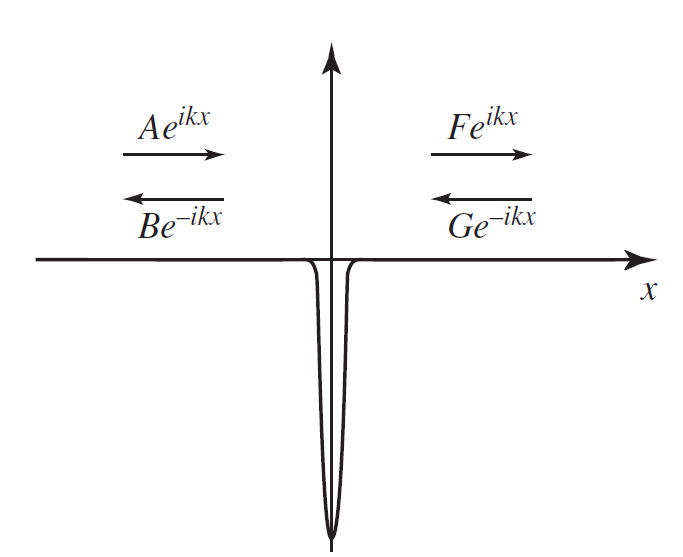
\includegraphics[width=0.5\linewidth]{./res/Pics/DeltaFunctionPotentialWaves.png}
    \caption{The four wave components of the solutions to the delta function potential.}
    \label{fig:DeltaFunctionPotentialWaves}
\end{figure}


\begin{itemize}
    \item From Fig.~\ref{fig:DeltaFunctionPotentialWaves}, we can see that for each region, there is a wave solution propagating left and right.
    \item In a normal experiment, in which we would be studying something like this, we would be firing particles from only one direction, say, from the left. Since there is no potential after the delta function well, there is now way for anything to come back, so we must have that $G=0$ (and we will typically know $A$ in advance, too).
    \item With this, we can now interpret $B$ as the amplitude of the \textbf{reflected wave}, and $C$ as the amplitude of the \textbf{transmitted wave}. Let's do a little bit of simplification:
        \begin{equation*}
            \begin{alignedat}{1}
            \begin{cases}
                C &= A+B, \\
                C &= A(1+2i\beta) - B(1-2i\beta).
            \end{cases}
            \end{alignedat}
        \end{equation*}
    \item We can solve for $B$ in terms of $A$:
        \begin{align*}
            A+B &= A(1+2i\beta) - B(1-2i\beta), \\
            0 &= 2A(i\beta) - 2B(1-i\beta), \\
            B(1-i\beta) &= Ai\beta, \\
            B &= \frac{i\beta}{1-i\beta}A.
        \end{align*}
        We can now solve for $C$ in terms of $A$:
        \begin{equation*}
            C = A\left( 1 + \frac{i\beta}{1-i\beta} \right) = \frac{1}{1-i\beta}A.
        \end{equation*}
    \item We can now examine the ratios of these amplitudes: \footnote{As a scattering state, we technically can't examine the probabilities in the same as if we were looking at bound states, since we know that individual stationary scattering states do not themselves form normalizable solutions. But since we are doing ratios here, this is okay.}
        \begin{equation}
            \boxed{R = \frac{\abs{B}^2}{\abs{A}^2} = \frac{\beta^2}{1 + \beta^2}.}
        \end{equation}
    \item $R$ is called the \textbf{reflection coefficient}, and it is the probability that the \textbf{incident wave} (whose amplitude is $A$) will reflect back. Similarly, the \textbf{transmission coefficent} $T$ is given by
        \begin{equation}
            \boxed{T = \frac{\abs{C}^2}{\abs{A}^2} = \frac{1}{1+\beta^2},}
        \end{equation}
        and it gives the probability that the incident waves transmits through the potential well.
    \item Additionally, we find that $R+T=1$, which is as expected.
    \item Now, since we know that $\beta$ is as well as what $k$ is, we can write
        \begin{equation}
            \boxed{R = \frac{1}{1+\frac{2\hbar^2 E}{m\alpha^2}},} \quad \mathrm{and} \quad \boxed{T = \frac{1}{1 + \frac{m\alpha^2}{2\hbar^2 E}}.}
        \end{equation}
\end{itemize}



\subsection*{The Finite Square Well}

\begin{itemize}
    \item Let's now revisit the infinite square well, but make it non-infinite. So, what we have now is
        \begin{equation}
            V(x) = 
                \begin{alignedat}{1}
                \begin{cases}
                    -V_0 \quad &\abs{x} <= a, \\
                    0 \quad &\abs{x} > a.
                \end{cases}
                \end{alignedat}
        \end{equation}
    \item From before, we know that this will permit both bound and scattering states; let's do the bound states first ($E<0$). First looking at the region $x < a$, we have no potential, so the SE reads
        \begin{equation*}
            -\frac{\hbar^2}{2m}\diff[2]{\psi}{x} = E\psi \rightarrow \diff[2]{\psi}{x} = k^2\psi,
        \end{equation*}
        where $k \equiv \frac{\sqrt{-2mE}}{\hbar}$ since $E$ is negative. This permits the solutions
        \begin{equation*}
            \psi(x) = Ae^{kx} + Be^{-kx}.
        \end{equation*}
        But the $B$ term blows up as $x \rightarrow -\infty$, so we only have 
        \begin{equation}
            \psi(x) = Ae^{kx} \quad \mathrm{for} \quad x<a.
        \end{equation}
    \item Similarly, for the region $x>a$, we will have similar solutions but the other term will blow up so
        \begin{equation}
            \psi(x) = Be^{-kx} \quad \mathrm{for} \quad x>a.
        \end{equation}
    \item Inside the well, we have
        \begin{equation*}
            -\frac{\hbar^2}{2m}\diff[2]{\psi}{x} -V_0\psi = E\psi \rightarrow \diff[2]{\psi}{x} = -\ell^2\psi,
        \end{equation*}
        where $\ell \equiv \frac{\sqrt{2m(V_0 + E)}}{2m}$. Since $E > -V_0$, then $E+V_0>0$ and $\ell$ is real, as required. This has solutions
        \begin{equation}
            \psi(x) = C\sin(lx) + D\cos(lx).
        \end{equation}
    \item Before we impose boundary conditions, let's consider the following statement: \textit{If $V(x)$ is an even function, then $\psi(x)$ can always be taken to be either even or odd}. To prove this, we first assume that we have a $\psi(x)$ that satisfies the SE. If we take $x \rightarrow -x$, then the SE becomes:
        \begin{equation*}
            -\frac{\hbar^2}{2m}\frac{\dd^2 \psi(-x)}{\dd (-x)^2} + V(-x)\psi(-x) = E\psi(-x).
        \end{equation*}
        Now obviously the differential $\dd (-x)^2 = \ddx^2$, and if $V$ is even, then $V(-x) = V(x)$, so we get
        \begin{equation*}
            -\frac{\hbar^2}{2m}\diff[2]{\psi}{x} + V(x)\psi(-x) = E\psi(-x).
        \end{equation*}
        We can see that we have retrieved the SE, but with $\psi(-x)$ instead, meaning that $\psi(-x)$ satisfies the SE just as well as $\psi(x)$. Then, since the Hamiltonian operator is a linear operator, then a linear combination of the two ($c_1\psi(x) + c_2\psi(-x)$) will also satisfy the SE.
    \item This is exactly what we have in this case: $V(x)$ is an even function, and we even have $\psi(x)$ inside the well in the perfect format to motivate taking either the even (cosine) or odd (sine) functions and have either (separately) still satisfy the SE. Let's do the evens part first, meaning we will drop the sine term. Continuity of $\psi$ at $x=a$ requires
        \begin{equation*}
            D\cos(\ell a) = Be^{-kx},
        \end{equation*}
        and the continuity of $\dd\psi/\ddx$ requires:
        \begin{equation*}
            -\ell D\sin(\ell a) = -kBe^{-kx}.
        \end{equation*}
        Dividing two, we get:
        \begin{equation}
            \ell\tan(\ell a) = k.
        \end{equation}
    \item Now, this does indeed give us the allowed energies, just like we did for previous cases. However, this is terribly hard to parse, so let's massage it a little bit. First, we define
        \begin{equation}
            z \equiv \ell a, \quad \mathrm{and} \quad z_0 = \frac{a}{\hbar}\sqrt{2mV_0}.
        \end{equation}
        Then, with a little bit of algebra, we can find
        \begin{equation}
            \tan z = \sqrt{\br{\frac{z_0}{z}}^2 - 1}.\label{eq:FiniteSquareWellEQ}
        \end{equation}
\end{itemize}


\begin{figure}[ht]
    \centering
    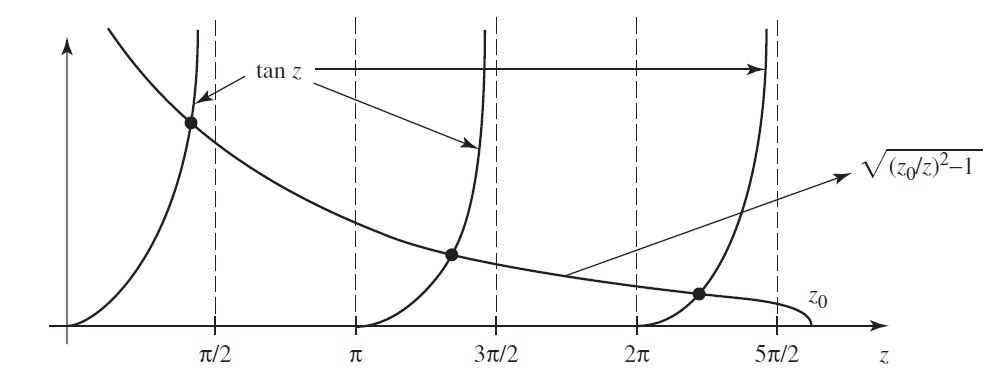
\includegraphics[width=0.66\textwidth]{./res/Pics/FiniteSquareWellEvenEnergies.png}
    \caption{Plots of either side of Eq.~\eqref{eq:FiniteSquareWellEQ}; the line crossing points are allowed values of energy.}
    \label{fig:FiniteSquareWellEvenEnergies}
\end{figure}



\begin{itemize}
    \item Now, these solutions on their own are not particularly illuminating. But we have two limiting cases that are kinda interesting. The first is when the well gets wide and/or deep; i.e. we increase $z_0$. This has the graphical effect of pushing the square root curve upwards and making it flatter. We can tell, then, that this would increase the number of solutions, and if we let $z_0 \rightarrow \infty$, we end up with an infinite number of solutions. We can also tell that those solutions would correspond to $z=n\pi/2$ for odd $n$:
        \begin{equation*}
            \frac{n\pi}{2} = z = la = a\frac{\sqrt{2m(E+V_0)}}{\hbar} \rightarrow E+V_0 = \frac{n^2\pi^2\hbar^2}{2m(2a)^2}.
        \end{equation*}
        This is exactly the infinite square well solutions with $a \rightarrow 2a$ and shifted by $V_0$. Well, that makes sense.
    \item The next case is the opposite we let the well get narrower/shallower. All that is involved with this one is that graphically, there will still be an intersection between the two curves regardless of how small $z_0$ becomes, meaning that there is always at least one bound state.
\end{itemize}

\begin{itemize}
    \item The odd solutions and scattering states aren't very illuminating. We didn't even do the former in class at all, and the latter was rushed because we went slow for the first bit of class. As a result, I'm not typing any of it out. Hopefully formalism is next!
\end{itemize}
%%% Local Variables:
%%% mode: LaTeX
%%% TeX-master: "../../Notes"
%%% End:
